\documentclass{article}

\usepackage{pgf}
\usepackage{tikz}
\usetikzlibrary{arrows,automata}
\usepackage[latin1]{inputenc}
\begin{document}

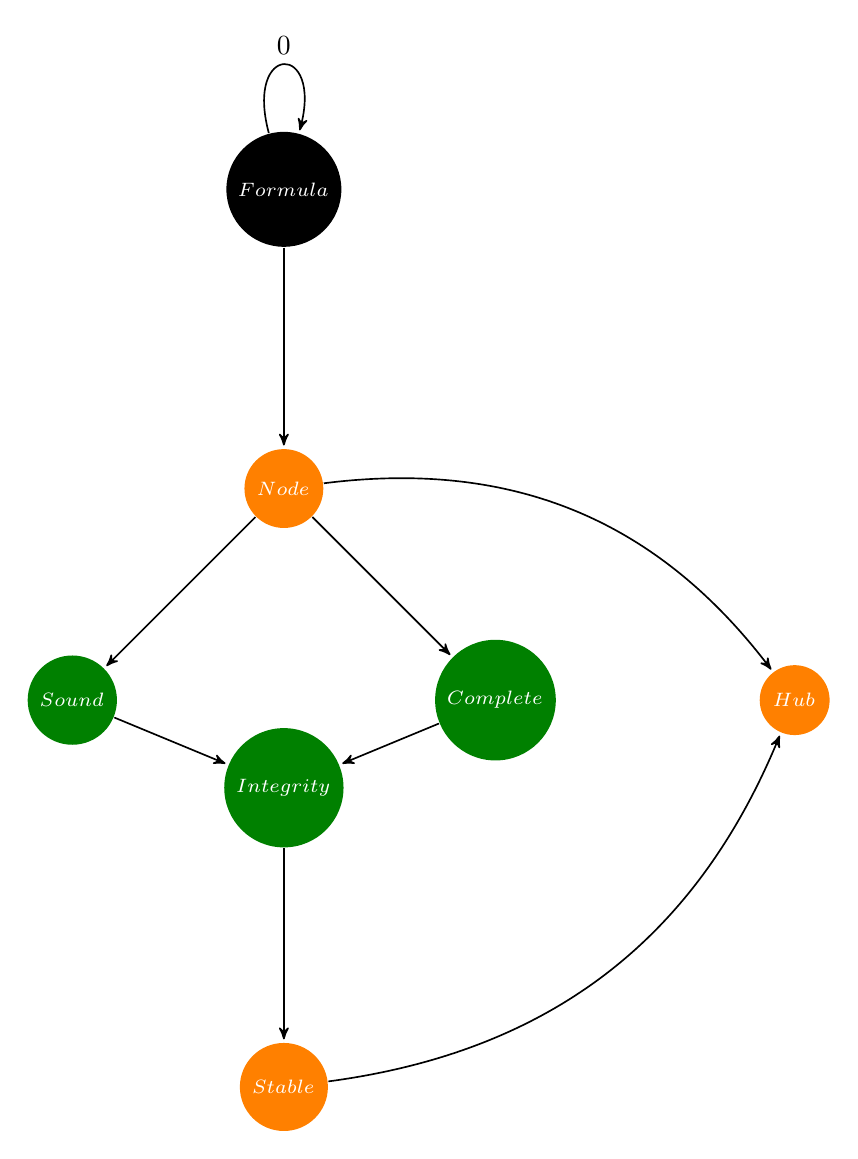
\begin{tikzpicture}[->,>=stealth',shorten >=1pt,auto,node distance=3.8cm,semithick]
  	\tikzstyle{every state}=[fill,draw=none,orange,text=white]
	\tikzstyle{validator}=[green!50!black,text=white]
	\tikzstyle{initial}= [black,text=white]

  \node[state,initial] 		(A)                     		{$_{Formula}$};
  \node[state]         			(B) [below of=A] 		{$_{Node}$};
  \node[state,validator]         	(C) [below left of=B] 	{$_{Sound}$};
  \node[state,validator]         	(D) [below right of=B] 	{$_{Complete}$};
  \node[state,validator]         	(E) [below of=B]       	{$_{Integrity}$};
  \node[state]         			(F) [below of=E]       	{$_{Stable}$};
  \node[state]         			(H) [right of=D]       		{$_{Hub}$};

  \path (A) edge    	node {} (B)
             edge [loop above] node {0} (A)          
        (B) edge 			node {} (C)
             edge 			node {} (D)
             edge [bend left] node {} (H)
        (C) edge		node {} (E)
        (D) edge		node {} (E)
        (E) edge		node {} (F)
	(F) edge [bend right] node {} (H);

\end{tikzpicture}

\end{document}